\section{Game Architecture}

%\begin{figure*}[!t]
%    \centering
%    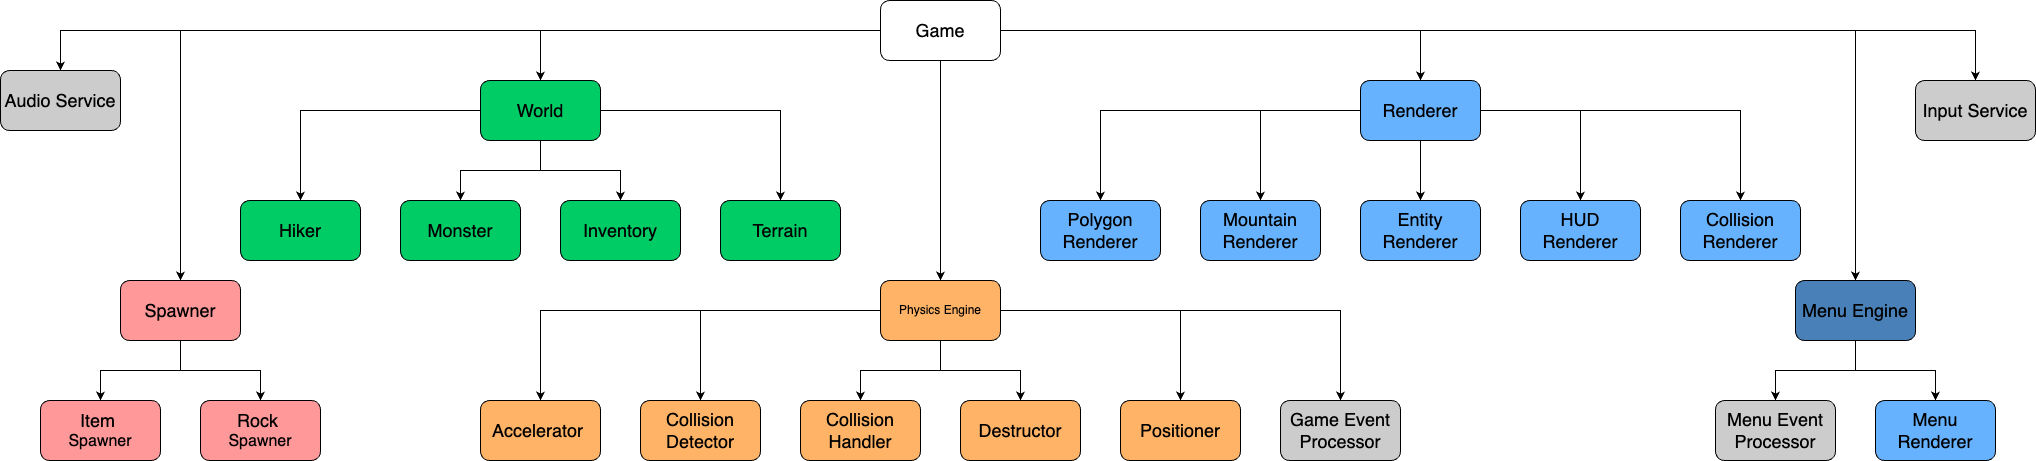
\includegraphics[scale=0.25]{figures/Architectural-Diagramm.drawio.png}
%    \caption{Architectural diagram}
%    \label{fig:architecture}
%\end{figure*}

The game is built using a highly modular architecture that allows for flexibility, scalability, and ease of maintenance.
The modular design breaks down the game into distinct components, each responsible for a specific functionality.
This approach ensures that different parts of the game can be developed, tested, and modified independently, making the overall system more manageable.
Below, we describe the general architecture and how different parts contribute to building the game.

\subsection{The Game Loop}\label{sec:gameLoop}

The game loop is the central control unit of our program and defines the interaction of the game's core components.
It contains all the logic and data needed to run the actual gameplay.
Our game loop is depicted in fig. \ref{fig:gameLoop}.
For the most part, it adheres to the industry standard as described by Nystrom \cite{nystromGameLoop} and the Unity framework \cite{unityGameLoop}.
Hence, we will only briefly describe its functionality here.

\begin{figure}[h!]
    \centering
    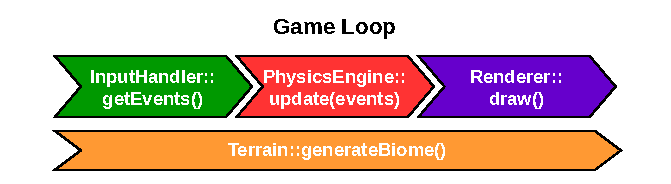
\includegraphics[width=\linewidth]{figures/physics/gameLoop.pdf}
    \caption{The game loop represents the fundamental structure of the game and comprises three distinct phases. The terrain generation is performed concurrently.}
    \label{fig:gameLoop}
\end{figure}

At the start of the game loop, input from the player, be it via keyboard or gamepad, is registered and passed to the physics engine.
The physics engine progresses the simulation in one or more constant time steps between frames (c.f. decoupling in sec. \ref{sec:decoupling}), thereby processing the collected input events.
Finally, the renderer draws the new frame representing the updated world state.

Due to the sequential nature of input receipt, input processing, simulating a physics step, and rendering the resulting new state of the world, the game loop is also inherently sequential.
For very large games or powerful frameworks such as the aforementioned Unity framework, a parallelization becomes inevitable, but in our game, this structure suffices.
As described in sec. \ref{sec:performance}, the physics engine does not have to run on a separate thread for our purpose.
Merely the terrain generation is extracted from the spawning phase of the physics engine in order to guarantee a smooth transition between biomes during gameplay.

\subsection{Core Components and Services}

The game is initialized through a \code{GameFactory} class, responsible for building and configuring all core components and dependencies.
These components can be categorized into services, game entities, menu systems, rendering pipelines, spawning systems, and the physics engine.

\subsection{Services}
Several core services are initialized within the \code{GameFactory} to manage resources, input, and audio:

\begin{itemize}
    \item \textbf{ConfigService:} A singleton pattern is used to handle game configuration (including YAML settings), ensuring game constants and configurations are readily available throughout the game.
    \item \textbf{InputService:} A singleton service responsible for managing input from various devices, such as gamepads and keyboards.
    \item \textbf{ResourceService:} Handles loading and management of game assets such as textures, audio, and other resources. It depends on the \code{ConfigManager} to load the assets specified in the YAML file.
    \item \textbf{AudioService:} Manages sound effects and background music. It interacts with the \code{ResourceManager} to load sound files and handle audio playback within the game.
    \item \textbf{DifficultyService:} A singleton service that manages the difficulty progression during the gameplay.
\end{itemize}

\subsection{Game Entities}

Key in-game entities, such as the terrain, hiker, and inventory, are created and managed by the \code{GameFactory}.
These entities interact with the world and with each other, providing the core gameplay functionality.

\begin{itemize}
    \item \textbf{Terrain:} Generated based on game constants and managed by the \code{Terrain} class. It determines the physical environment in which the player interacts.
    \item \textbf{Hiker:} The main player character, represented by the \code{Hiker} class.
    \item \textbf{Monster:} An antagonist entity represented by the \code{Monster} class, which adds an element of challenge for the player, acting as a threat.
    \item \textbf{Inventory:} Manages the player's items and inventory.
\end{itemize}

These entities are bound together within the \code{World} class, which encapsulates the terrain, hiker, monster, and inventory, managing their interactions.


\subsection{Spawner System}

The game includes a system for dynamically spawning items and rocks during gameplay:

\begin{itemize}
    \item \textbf{ItemSpawner:} Spawns items in the world based on configuration from the YAML file (e.g., item spawn rates and types).
    \item \textbf{RockSpawner:} Dynamically spawns rocks of various sizes, speeds, and densities during gameplay, adding an element of challenge.
    \item \textbf{Spawner:} A unified spawner that manages both the \code{ItemSpawner} and \code{RockSpawner}. It also initiates the terrain generation.
\end{itemize}

This modular spawner system allows for dynamic game elements that can evolve based on player progress or difficulty.
\pagebreak
\subsection{Physics and Collision Detection}

The game incorporates a robust physics engine to handle movement, collisions, and interactions between entities:

\begin{itemize}
    \item \textbf{Accelerator:} Applies acceleration forces to the entities to the hiker and other objects in the game world. So far, only gravitational forces are considered.
    \item \textbf{CollisionDetector:} Detects collisions between entities (e.g., hiker and terrain, rocks, or inventory items) to trigger corresponding responses.
    \item \textbf{CollisionHandler:} Handles the game logic triggered by collisions, such as taking damage or picking up items.
    \item \textbf{Destructor:} Handles the accurate and timely destruction of entities.
    \item \textbf{Positioner:} Handles the correct positioning of the entities within the game
    \item \textbf{PhysicsEngine:} The central physics engine that manages all other physics modules.
\end{itemize}
By abstracting collision detection and handling into separate classes, the game ensures that its physics are flexible and can easily be adapted or expanded upon.

\subsection{Menus and UI}

The game uses a sophisticated menu system to handle the user interface, including in-game menus. This system is composed of:

\begin{itemize}
    \item \textbf{MenuEngine:} Responsible for managing the game's various menus, including the start screen, settings, and pause menus. It also handles user input in these menus.
    \item \textbf{FullMenuRenderer:} Renders the menu components on the screen.
    \item \textbf{MenuEventProcessor:} Handles events that occur within the menus, such as button clicks and navigation.
\end{itemize}

This system ensures that the menu and UI are distinct from the core game logic, allowing independent development and modification of the user interface.

\subsection{Renderer}

The game rendering is divided into several subsystems to ensure modular and efficient drawing of different elements:

\begin{itemize}
    \item \textbf{PolygonRenderer:} Used for drawing polygonal shapes, typically for terrain or other geometric elements.
    \item \textbf{MountainRenderer:} A specialized renderer for drawing the mountain and environmental elements in the background.
    \item \textbf{EntityRenderer:} Handles rendering of game entities (e.g., the hiker, inventory items, and the monster).
    \item \textbf{HUDRenderer:} Renders the HUD, displaying information such as health, score, and inventory status.
    \item \textbf{Renderer:} The central renderer that coordinates all these subsystems. It integrates the \code{World} entities and renders the terrain, entities, and HUD together.
\end{itemize}

This modular rendering system separates concerns, ensuring that changes to how entities are drawn, or the addition of new visual elements, can be done without affecting the rest of the game.